\paragraph{QuizziPedia::Back-End::App::Controllers::QuizController}
\label{QuizziPedia::Back-End::App::Controllers::QuizController}
\begin{figure}[ht]
	\centering
	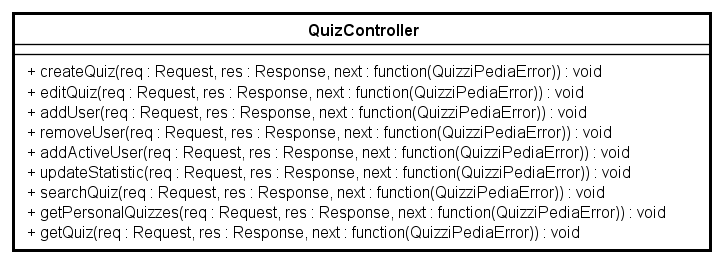
\includegraphics[scale=0.8]{UML/Classi/Back-End/QuizziPedia_Back-End_App_Controllers_quizController.png}
	\caption{QuizziPedia::Back-End::App::Models::Controllers::TopicController}
\end{figure}
\FloatBarrier

\begin{itemize}
	\item \textbf{Descrizione}:
	classe che gestisce la logica applicativa riguardante la visualizzazione e la gestione dei questionari.;
	\item \textbf{Utilizzo}:
	viene utilizzata per implementare le funzionalità necessarie a gestire le richieste \textit{REST\ped{G}} legate alla gestione dei questionari;
	\item \textbf{Relazione con altre classi}:
	\begin{itemize}
			\item \textbf{IN \texttt{QuizRouter}}:
			classe che gestisce le richieste relative alle operazioni riguardanti un questionario;
			\item \textbf{OUT \texttt{QuizModel}}:
			classe che modella i questionari.
	\end{itemize}
	\item \textbf{Metodi}:
	\begin{itemize}
		\item \texttt{+ createQuiz(req: Request, res: Response, \\next: function(QuizziPediaError)): void}\\
		Crea un questionario.\\
		\textbf{Parametri}:
		\begin{itemize}
			\item \texttt{req: Request}\\
			Rappresenta la richiesta inviata al \textit{server\ped{G}}. Contiene i dati che verranno utilizzati per creare il questionario e gli identificativi delle domande che verranno inserite;
			\item \texttt{res: Response}\\
			Rappresenta la risposta che il \textit{server\ped{G}} fornirà al termine dell'esecuzione del metodo;
			\item \texttt{next: function(QuizziPediaError)}\\
			Rappresenta la \textit{callback\ped{G}} che il metodo deve chiamare al termine dell'elaborazione per passare il controllo ai successivi \textit{middleware\ped{G}}. La presenza del parametro facoltativo \texttt{QuizziPediaError} attiva la catena di gestione dell'errore in sostituzione della normale catena di gestione delle richieste.
		\end{itemize}
	
	\item \texttt{+ editQuiz(req: Request, res: Response, \\next: function(QuizziPediaError)): void}\\
		Modifica un questionario secondo i dati inseriti dall'utente.\\
		\textbf{Parametri}:
		\begin{itemize}
			\item \texttt{req: Request}\\
			Rappresenta la richiesta inviata al \textit{server\ped{G}}. Contiene le modifiche apportate dall'utente e l'identificativo del questionario su cui verranno applicate;
			\item \texttt{res: Response}\\
			Rappresenta la risposta che il \textit{server\ped{G}} fornirà al termine dell'esecuzione del metodo;
			\item \texttt{next: function(QuizziPediaError)}\\
			Rappresenta la \textit{callback\ped{G}} che il metodo deve chiamare al termine dell'elaborazione per passare il controllo ai successivi \textit{middleware\ped{G}}. La presenza del parametro facoltativo \texttt{QuizziPediaError} attiva la catena di gestione dell'errore in sostituzione della normale catena di gestione delle richieste.
		\end{itemize}
		
		\item \texttt{+ addUser(req: Request, res: Response, \\next: function(QuizziPediaError)): void}\\
		Iscrive un utente al questionario.\\
		\textbf{Parametri}:
		\begin{itemize}
			\item \texttt{req: Request}\\
			Rappresenta la richiesta inviata al \textit{server\ped{G}}. Contiene l'identificativo del questionario la cui lista delle iscrizioni deve essere modificata;
			\item \texttt{res: Response}\\
			Rappresenta la risposta che il \textit{server\ped{G}} fornirà al termine dell'esecuzione del metodo;
			\item \texttt{next: function(QuizziPediaError)}\\
			Rappresenta la \textit{callback\ped{G}} che il metodo deve chiamare al termine dell'elaborazione per passare il controllo ai successivi \textit{middleware\ped{G}}. La presenza del parametro facoltativo \texttt{QuizziPediaError} attiva la catena di gestione dell'errore in sostituzione della normale catena di gestione delle richieste.
		\end{itemize}
		\item \texttt{+ removeUser(req: Request, res: Response, \\next: function(QuizziPediaError)): void}\\
		Disiscrive un utente al questionario.\\
		\textbf{Parametri}:
		\begin{itemize}
			\item \texttt{req: Request}\\
			Rappresenta la richiesta inviata al \textit{server\ped{G}}. Contiene l'identificativo del questionario la cui lista delle iscrizioni deve essere modificata;
			\item \texttt{res: Response}\\
			Rappresenta la risposta che il \textit{server\ped{G}} fornirà al termine dell'esecuzione del metodo;
			\item \texttt{next: function(QuizziPediaError)}\\
			Rappresenta la \textit{callback\ped{G}} che il metodo deve chiamare al termine dell'elaborazione per passare il controllo ai successivi \textit{middleware\ped{G}}. La presenza del parametro facoltativo \texttt{QuizziPediaError} attiva la catena di gestione dell'errore in sostituzione della normale catena di gestione delle richieste.
		\end{itemize}
		
		\item \texttt{+ addActiveUser(req: Request, res: Response, \\next: function(QuizziPediaError)): void}\\
		Aggiorna la lista di utenti che hanno svolto il questionario.\\
		\textbf{Parametri}:
		\begin{itemize}
			\item \texttt{req: Request}\\
			Rappresenta la richiesta inviata al \textit{server\ped{G}}. Contiene l'identificativo del questionario la cui lista delle iscrizioni deve essere modificata;
			\item \texttt{res: Response}\\
			Rappresenta la risposta che il \textit{server\ped{G}} fornirà al termine dell'esecuzione del metodo;
			\item \texttt{next: function(QuizziPediaError)}\\
			Rappresenta la \textit{callback\ped{G}} che il metodo deve chiamare al termine dell'elaborazione per passare il controllo ai successivi \textit{middleware\ped{G}}. La presenza del parametro facoltativo \texttt{QuizziPediaError} attiva la catena di gestione dell'errore in sostituzione della normale catena di gestione delle richieste.
		\end{itemize}
		
		\item \texttt{+ updateStatistic(req: Request, res: Response, \\next: function(QuizziPediaError)): void}\\
		Aggiorna le statistiche del questionario.\\
		\textbf{Parametri}:
		\begin{itemize}
			\item \texttt{req: Request}\\
			Rappresenta la richiesta inviata al \textit{server\ped{G}}. Contiene l'identificativo del questionario le cui statistiche dovranno essere modificate e i valori da aggiornare;
			\item \texttt{res: Response}\\
			Rappresenta la risposta che il \textit{server\ped{G}} fornirà al termine dell'esecuzione del metodo;
			\item \texttt{next: function(QuizziPediaError)}\\
			Rappresenta la \textit{callback\ped{G}} che il metodo deve chiamare al termine dell'elaborazione per passare il controllo ai successivi \textit{middleware\ped{G}}. La presenza del parametro facoltativo \texttt{QuizziPediaError} attiva la catena di gestione dell'errore in sostituzione della normale catena di gestione delle richieste.
		\end{itemize}
		
		\item \texttt{+ searchQuiz(req: Request, res: Response, \\next: function(QuizziPediaError)): void}\\
		Ricerca un questionario.\\
		\textbf{Parametri}:
		\begin{itemize}
			\item \texttt{req: Request}\\
			Rappresenta la richiesta inviata al \textit{server\ped{G}}. Contiene il nome del questionario da ricercare;
			\item \texttt{res: Response}\\
			Rappresenta la risposta che il \textit{server\ped{G}} fornirà al termine dell'esecuzione del metodo;
			\item \texttt{next: function(QuizziPediaError)}\\
			Rappresenta la \textit{callback\ped{G}} che il metodo deve chiamare al termine dell'elaborazione per passare il controllo ai successivi \textit{middleware\ped{G}}. La presenza del parametro facoltativo \texttt{QuizziPediaError} attiva la catena di gestione dell'errore in sostituzione della normale catena di gestione delle richieste.
		\end{itemize}
		
		\item \texttt{+ getPersonalQuizzes((req: Request, res: Response, \\next: function(QuizziPediaError)): void}\\
			Mostra i questionari creati da un utente.\\
			\textbf{Parametri}:
			\begin{itemize}
				\item \texttt{req: Request}\\
			Rappresenta la richiesta inviata al \textit{server\ped{G}}. Contiene l'identificativo dell'utente che ha creato i questionari da visualizzare;
				\item \texttt{res: Response}\\
			Rappresenta la risposta che il \textit{server\ped{G}} fornirà al termine dell'esecuzione del metodo;
				\item \texttt{next: function(QuizziPediaError)}\\
			Rappresenta la \textit{callback\ped{G}} che il metodo deve chiamare al termine dell'elaborazione per passare il controllo ai successivi \textit{middleware\ped{G}}. La presenza del parametro facoltativo \texttt{QuizziPediaError} attiva la catena di gestione dell'errore in sostituzione della normale catena di gestione delle richieste.
			\end{itemize}
			
			\item \texttt{+ getQuiz((req: Request, res: Response, \\next: function(QuizziPediaError)): void}\\
			Mostra il questionario da compilare.\\
			\textbf{Parametri}:
			\begin{itemize}
				\item \texttt{req: Request}\\
			Rappresenta la richiesta inviata al \textit{server\ped{G}}. Contiene l'identificativo del questionario da compilare;
				\item \texttt{res: Response}\\
			Rappresenta la risposta che il \textit{server\ped{G}} fornirà al termine dell'esecuzione del metodo;
				\item \texttt{next: function(QuizziPediaError)}\\
			Rappresenta la \textit{callback\ped{G}} che il metodo deve chiamare al termine dell'elaborazione per passare il controllo ai successivi \textit{middleware\ped{G}}. La presenza del parametro facoltativo \texttt{QuizziPediaError} attiva la catena di gestione dell'errore in sostituzione della normale catena di gestione delle richieste.
			\end{itemize}
	\end{itemize}		
\end{itemize}